% SC4013 --- Chapter 7: Security Testing, SAST/DAST, ZAP/Burp and Pentest Methodology (0->100 ground-up)
\chapter{Security Testing, SAST/DAST, ZAP/Burp and Pentest Methodology}
\label{ch:testing}

\begin{quote}
\emph{``Tests prove the presence of features; security tests prove the absence of certain bugs.''} --- SAST reads the code, DAST attacks the running app, and a pentest tells the story of how an adversary would chain them.
\end{quote}

\noindent\fbox{\parbox{\dimexpr\linewidth-2\fboxsep-2\fboxrule}{%
\textbf{From zero: how testing differs for security.} We start from unit tests, show why they miss injection and auth flaws, then build SAST/DAST/IAST, hands-on ZAP and Burp, and a methodology that turns findings into a report. No prior security-testing background assumed.}}
\vspace{0.4em}

\section*{Learning Outcomes}
After this chapter you will be able to:
\begin{enumerate}[label=(L\arabic*)]
    \item contrast SAST, DAST, IAST and SCA and when each applies;
    \item run ZAP and Burp Suite to find XSS, SQLi and auth flaws;
    \item describe PTES/OSSTMM methodology and rules of engagement;
    \item triage findings (true vs.\ false positive, severity with CVSS);
    \item write a pentest report with reproduction, impact and fix guidance.
\end{enumerate}

% ============================================================
\section{SAST, DAST, IAST and SCA}
\label{sec:sast-dast}
Intuition: SAST (Static Application Security Testing) reads source/bytecode without running it, like a linter with a security rulebook. DAST (Dynamic) attacks the running app over HTTP, like an outsider. IAST (Interactive) instruments the app at runtime and watches data flow. SCA (Software Composition Analysis) flags known CVEs in dependencies.

\begin{figure}[h]\centering
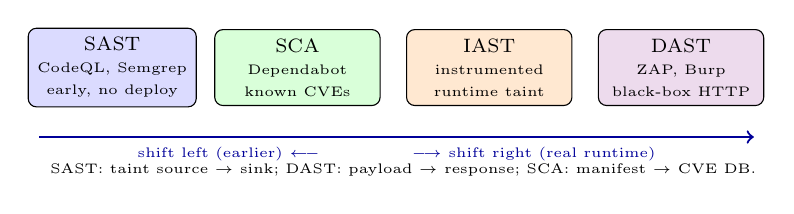
\begin{tikzpicture}[scale=0.84,every node/.style={font=\scriptsize}]
  \node[draw,fill=blue!14,rounded corners=3pt,minimum width=2.1cm,minimum height=0.8cm,align=center] (sast) at (-4.4,1.6) {SAST\\\tiny CodeQL, Semgrep\\\tiny early, no deploy};
  \node[draw,fill=green!15,rounded corners=3pt,minimum width=2.1cm,minimum height=0.8cm,align=center] (sca) at (-1.6,1.6) {SCA\\\tiny Dependabot\\\tiny known CVEs};
  \node[draw,fill=orange!18,rounded corners=3pt,minimum width=2.1cm,minimum height=0.8cm,align=center] (iast) at (1.3,1.6) {IAST\\\tiny instrumented\\\tiny runtime taint};
  \node[draw,fill=violet!14,rounded corners=3pt,minimum width=2.1cm,minimum height=0.8cm,align=center] (dast) at (4.2,1.6) {DAST\\\tiny ZAP, Burp\\\tiny black-box HTTP};
  \draw[->,thick,blue!60!black] (-5.5,0.55) -- (5.3,0.55) node[midway,below,font=\tiny] {shift left (earlier) $\longleftarrow$ \hspace{1cm} $\longrightarrow$ shift right (real runtime)};
  \node[font=\tiny,align=center] at (0,0.05) {SAST: taint source $\to$ sink; DAST: payload $\to$ response; SCA: manifest $\to$ CVE DB.};
\end{tikzpicture}
\caption{Testing quadrant. SAST/SCA run in CI on every commit; IAST in test; DAST against staging. No single quadrant covers all bug classes.}
\label{fig:testing-quad}
\end{figure}

SAST strength: finds taint flows (\texttt{request.getParam()} $\to$ \texttt{SQL.execute()}), hard-coded secrets, weak crypto. Weakness: false positives, needs language support. DAST strength: finds what is actually exploitable over HTTP (XSS, auth bypass). Weakness: needs a running app, misses code not reachable via crawl. IAST bridges both but needs agent deployment.

\begin{lstlisting}[language=Python]
# SAST intuition: taint rule (Semgrep-style) for SQLi
# rule: pattern: cursor.execute("SELECT ..."+ $INPUT)  -> flag
#       pattern-not: cursor.execute("SELECT ... WHERE id=?", ($INPUT,))
# SAST reports: "Untrusted input $INPUT reaches SQL sink without parameterisation"
# Developer fixes by binding parameters; SAST re-runs green in CI.

# DAST intuition: ZAP active scan payloads
# GET /search?q=<script>alert(1)</script>  -> reflect? => XSS
# GET /api/users/43  with other user's token -> 200? => BOLA
\end{lstlisting}

Triage: SAST flags are ``maybes'' until a sink is confirmed reachable; DAST flags are ``witnessed'' but may miss auth-gated paths without a valid session. Gate CI on high-confidence SAST rules; run DAST nightly on staging with seeded users/roles.

% ============================================================
\section{ZAP and Burp Suite in Practice}
\label{sec:zap-burp}
OWASP ZAP (free) and Burp Suite (Community/Pro) are intercepting proxies: the browser (or API client) routes through them; they see and modify every request/response.

Workflow: (1)~spider/crawl to discover routes, (2)~passive scan (headers, cookies), (3)~active scan (inject payloads), (4)~manual intrude/repeat for logic flaws.

\begin{figure}[h]\centering
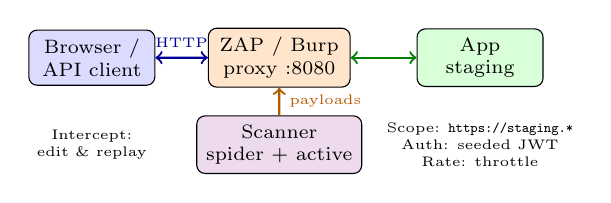
\begin{tikzpicture}[scale=0.85,every node/.style={font=\scriptsize}]
  \node[draw,fill=blue!14,rounded corners=3pt,minimum width=1.6cm,minimum height=0.7cm,align=center] (browser) at (-4.2,1.4) {Browser /\\API client};
  \node[draw,fill=orange!20,rounded corners=3pt,minimum width=1.8cm,minimum height=0.7cm,align=center] (proxy) at (-1.4,1.4) {ZAP / Burp\\proxy :8080};
  \node[draw,fill=green!15,rounded corners=3pt,minimum width=1.6cm,minimum height=0.7cm,align=center] (app) at (1.6,1.4) {App\\staging};
  \node[draw,fill=violet!14,rounded corners=3pt,minimum width=1.8cm,minimum height=0.7cm,align=center] (scan) at (-1.4,0.1) {Scanner\\spider + active};
  \draw[<->,thick,blue!60!black] (browser) -- (proxy) node[midway,above,font=\tiny] {HTTP};
  \draw[<->,thick,green!50!black] (proxy) -- (app);
  \draw[->,thick,orange!70!black] (scan) -- (proxy) node[midway,right,font=\tiny] {payloads};
  \node[font=\tiny,align=center] at (1.6,0.1) {Scope: \texttt{https://staging.*}\\Auth: seeded JWT\\Rate: throttle};
  \node[font=\tiny,align=center] at (-4.2,0.1) {Intercept:\\edit \& replay};
\end{tikzpicture}
\caption{Proxy-based DAST. The proxy sees plaintext HTTP, can spider the app, inject payloads, and replay with modified auth/params.}
\label{fig:proxy-dast}
\end{figure}

ZAP quick start: \texttt{zap.sh -cmd -quickurl https://staging.example.com -quickout report.html}. In the UI, set Context (include scope, auth via script), run Spider then Active Scan, then check Alerts (ranked High/Med/Low). Burp: set browser proxy to \texttt{127.0.0.1:8080}, install CA cert, use Intruder to brute-force \texttt{id} for BOLA, Repeater to tweak \texttt{alg} in a JWT, and Collaborator to detect SSRF.

\begin{lstlisting}[language=Python]
# Automating ZAP via its API (python-owasp-zap-v2)
from zapv2 import ZAPv2
zap = ZAPv2(proxies={"http":"http://127.0.0.1:8080","https":"http://127.0.0.1:8080"})
zap.spider.scan("https://staging.example.com")
while int(zap.spider.status()) < 100: pass
zap.ascan.scan("https://staging.example.com")
while int(zap.ascan.status()) < 100: pass
for alert in zap.core.alerts(baseurl="https://staging.example.com"):
    print(alert["risk"], alert["alert"], alert["url"])
\end{lstlisting}

Manual testing still owns logic flaws (BOLA, BFLA, mass assignment) that scanners miss because they require understanding of ``who should own what.'' Seed two test users (alice, bob) and replay alice's request with bob's token; a 200 is the finding.

% ============================================================
\section{Coverage, False Positives and IAST/SCA Integration}
\label{sec:coverage}
SAST coverage is limited by language and framework support; it also suffers false positives when a tainted path is not actually reachable (dead code, validated upstream). Tune rules: disable noisy low-confidence rules in CI, keep high-confidence injection/auth rules as blockers, and track false-positive rate per rule to guide customisation.

IAST shines where SAST and DAST are blind: it observes the actual runtime data flow inside the app (the same taint \texttt{source $\to$ sink} as SAST, but confirmed at runtime) and reports with a full stack trace and HTTP request. Deploy the IAST agent in the test environment, run functional tests, and collect findings that include ``this parameter reached this query without sanitisation.'' SCA is orthogonal: it flags that you ship \texttt{log4j 2.14.1} with CVE-2021-44228, regardless of whether your code calls the vulnerable JNDI lookup. Pair SCA with reachability (does your call graph hit the vulnerable method?) to prioritise.

\begin{example}[Tuning SAST in CI]
Start with Semgrep or CodeQL high-precision rules: secrets, SQLi, XSS sinks, weak crypto. Gate PRs on those. Run the full rule pack nightly and review as tech debt. Measure \emph{signal}: number of true positives fixed per week vs.\ number of ignored alerts. If developers ignore SAST, the rule set is too noisy---fix the rules, not the developers.
\end{example}

\begin{remark}[Threat-model-driven testing]
A threat model tells you \emph{what to test}. For ``export CSV'' the STRIDE was Tampering (filter bypass), Information Disclosure (cross-tenant), DoS (large export). Derive tests directly: tamper \texttt{tenant\_id} in the filter, request another tenant's ID, and request \texttt{limit=1M}. This maps threats to ZAP/Burp checks and to SAST rules that verify the tenant guard reaches the query.
\end{remark}

\begin{example}[SCA reachability]
Dependabot flags \texttt{lodash 4.17.20} with prototype pollution. If your code never calls \texttt{\_.merge} with attacker-controlled keys, the CVE may not be exploitable in your app---but it is still a liability (future code may call it, audit will flag it). Policy: fix reachable High immediately, schedule unreachable Medium/High in the next sprint, and never ship with a known Critical without a waiver signed by security.
\end{example}

\subsection{Triage, Severity and Reporting}
Triage answers ``is it real, how bad, how to fix.'' Reproduce with the exact request (proxy history, curl) and verify on a clean staging env. Severity: CVSS base plus environmental (is the asset the payment DB or an internal wiki?) and exploit maturity (public PoC? wormable?). A reflected XSS with a WAF bypass outranks a theoretical SAST flag with no sink.

The report is the pentest's product. Structure: executive summary (risk in business terms), scope/RoE, methodology (PTES phases, tools, coverage), findings table (ID, title, CVSS, severity, status), then per-finding pages: description, repro steps, evidence (screenshots, ZAP alert, HTTP trace), impact (what an attacker gains), fix (code diff or config), and references (OWASP, CVE). Append raw tool output and the scope doc. A finding without a repro is not a finding; a fix without a regression test will regress.

\begin{remark}[Continuous testing]
Pentests are snapshots; CI is continuous. Run ZAP baseline scan and SCA on every PR, full ZAP + IAST nightly, and a manual focused test per feature. Track metrics: mean-time-to-fix by severity, repeat-bug rate, and SAST true-positive rate. A flat alert count with falling coverage means the app grew faster than the tests.
\end{remark}

\begin{example}[Example finding: BOLA in the wild]
Title: BOLA on \texttt{GET /api/v1/invoices/\{id\}} (High, CVSS 8.1). Repro: as bob (\texttt{jwt=bob}), \texttt{GET /api/v1/invoices/1024} (alice's invoice) returns 200 with \texttt{\{amount: 5000, ssn: ...\}}. Evidence: Burp Repeater screenshot, ZAP alert ``IDOR''. Impact: any authenticated user reads any invoice, PII leak, GDPR breach. Fix: add per-object check \texttt{if invoice.owner != caller: 403} and add CodeQL taint rule + negative test \texttt{bob\_cannot\_get\_alice}. Regression: add to CI with two users.
\end{example}

\begin{remark}[Legal and ethical guardrails]
Never test without written authorisation. Scope excludes production data exfiltration, DoS, and social engineering unless explicitly included. Retain logs for the report, then purge sensitive data per the RoE. An unauthorised ``helpful'' scan is indistinguishable from an attack and may violate CFAA or local law.
\end{remark}

\begin{remark}[Bug bounty vs.\ pentest]
A pentest is time-boxed and exhaustive within scope; a bug bounty is continuous and incentive-driven but noisy. Use pentests for compliance and deep logic flaws, bounties for breadth and fresh eyes. Both need the same RoE discipline and triage pipeline; a bounty without SLA for fix is just a vulnerability feed.
\end{remark}

\begin{example}[OWASP WSTG checklist in CI]
Map WSTG tests to automation: WSTG-INPV-05 (SQLi) $\to$ SAST taint + DAST payload, WSTG-ATHN-01 (weak password policy) $\to$ config scan, WSTG-SESS-02 (cookie flags) $\to$ ZAP passive scan. Track WSTG coverage per release so gaps are visible.
\end{example}

% ============================================================
\section{Pentest Methodology and Rules of Engagement}
\label{sec:pentest}
A pentest is a scoped, authorised simulation of an adversary. PTES (Penetration Testing Execution Standard) defines seven phases: pre-engagement, intelligence gathering, threat modelling, vulnerability analysis, exploitation, post-exploitation, and reporting. OSSTMM and OWASP WSTG/ASTG give checklists per target class.

\begin{figure}[h]\centering
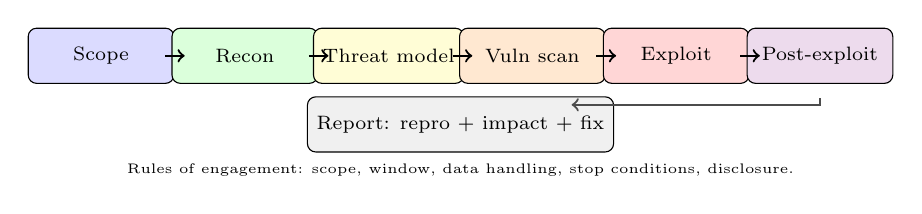
\begin{tikzpicture}[scale=0.83,every node/.style={font=\scriptsize}]
  \foreach \i/\lab/\col in {0/Scope/blue!14, 2.2/Recon/green!14, 4.4/Threat model/yellow!16, 6.6/Vuln scan/orange!18, 8.8/Exploit/red!16, 11.0/Post-exploit/violet!14} {
    \node[draw,fill=\col,rounded corners=3pt,minimum width=1.85cm,minimum height=0.7cm,align=center] at (\i,1.2) {\lab};
    \ifdim \i pt > 0pt \draw[->,thick] (\i-1.22,1.2) -- (\i-0.92,1.2); \fi
  }
  \node[draw,fill=gray!12,rounded corners=3pt,minimum width=3.0cm,minimum height=0.7cm,align=center] at (5.5,0.15) {Report: repro + impact + fix};
  \draw[->,thick,gray!60!black] (11.0,0.55) |- (7.2,0.45);
  \node[font=\tiny,align=center] at (5.5,-0.55) {Rules of engagement: scope, window, data handling, stop conditions, disclosure.};
\end{tikzpicture}
\caption{PTES phases. Each phase has an artefact (scope doc, recon map, threat model, scan report, proof, lessons). Skipping recon yields blind exploitation.}
\label{fig:ptes}
\end{figure}

Rules of engagement (RoE) are mandatory: scope (hosts/APIs in/out), window, rate limits, data handling (no real PII exfiltration), and stop conditions. Unscoped scanning is a crime in many jurisdictions. Record every command (proxy history, ZAP report) for reproducibility.

Severity uses CVSS plus business impact; a Medium on the payment flow outranks a High on an internal tool. The report must contain: executive summary, scope/RoE, methodology, findings (each with repro, evidence, CVSS, impact, fix, references), and an appendix of raw tool output.

\begin{example}[Scope creep and stop conditions]
A tester discovers a staging S3 bucket with prod backups outside the agreed scope. Continuing without approval violates the RoE and may breach data-handling clauses. The correct action: pause, document, notify the client contact, and only proceed after a signed scope amendment. The stop condition ``exposure of real PII'' triggers immediate halt and secure deletion.
\end{example}

\begin{remark}[Evidence hygiene]
Evidence must be reproducible: include the exact curl or Repeater request, the ZAP alert ID, and the response diff (200 vs.\ 403). Redact real tokens and PII in the report appendix; store the unredacted capture in the client's secure vault, not in the report PDF that will be emailed.
\end{remark}

\begin{remark}[Retesting and regression]
Every High/Critical finding needs a retest after the fix on a fresh staging build, plus a regression test that lives in CI (the repro request with the correct token should now return 403, the JWT with \texttt{alg:none} should return 401). Close a finding only after the retest passes and the regression is green; otherwise the bug will return with the next feature.
\end{remark}

% ============================================================
\section{Exercises}
\label{sec:ch07-exercises}
\begin{enumerate}[label=E7.\arabic*, leftmargin=*, itemsep=0.6em]
    \item \textbf{SAST vs.\ DAST.} For each bug --- reflected XSS, hard-coded AWS key, BOLA, weak JWT secret, SQLi via string concat --- state which of SAST/DAST/SCA is most likely to catch it and why. Which needs both?
    \item \textbf{ZAP session.} You are given \texttt{https://staging.example.com} with seeded users alice/bob. List the exact ZAP steps (context, auth script, spider, active scan) to test BOLA on \texttt{GET /api/users/\{id\}}. What response distinguishes pass from fail?
    \item \textbf{Burp intruder.} Design a Burp Intruder attack that tests mass assignment on \texttt{PUT /api/me} with payloads \texttt{role, is\_admin, balance}. Show the request template, payload positions, and how you detect success (reflect vs.\ DB check).
    \item \textbf{RoE drafting.} Draft a one-page RoE for a 2-day external pentest of a fintech API: scope (prod vs.\ staging), window, forbidden actions (DoS, social engineering), data handling, and disclosure timeline. Justify each clause.
    \item \textbf{Report writing.} Write a finding for a stored XSS in a comment field (repro curl, ZAP alert, CVSS 7.2 vector, impact, fix with output encoding + CSP nonce, and regression test). What evidence would you attach?
\end{enumerate}

\begin{remark}[Retest discipline]
A fix without a retest is not a fix. Re-run the exact DAST payload that triggered the finding, plus a variant (different encoding, different parameter). Add the payload to the regression corpus so CI fails if the fix regresses. Track retest pass rate as a metric for remediation quality.
\end{remark}

\begin{remark}[Coverage gaps]
SAST and DAST miss different things: SAST misses framework sinks that are not modelled (e.g., custom file-upload handler), DAST misses auth-gated paths without valid sessions. Close gaps with custom Semgrep rules for your sinks and ZAP scripts seeded with valid JWTs for each role. Measure coverage per trust boundary, not per URL count.
\end{remark}

\begin{example}[File upload path traversal]
A service does \texttt{open("uploads/" + filename)} where \texttt{filename} comes from a multipart upload. DAST payload \texttt{filename=../../etc/passwd} succeeds, but SAST reported 0 because the sink was inside a third-party library. Fix: add a taint rule for that library's file-write sink and a ZAP active scan that fuzzes \texttt{filename} with dot-dot payloads.
\end{example}

\section*{Chapter Notes}
SAST/DAST/IAST taxonomy follows Gartner and NIST SP 800-53; OWASP WSTG (Web Security Testing Guide) and MSTG (Mobile) are the practitioner checklists. ZAP is OWASP Flagship; Burp Suite is PortSwigger. PTES and OSSTMM define methodology; CVSS v3.1 (FIRST) scores severity. Reporting guidance follows PTES Technical Guidelines and OWASP ASVS.

% End of Chapter 7
